\documentclass[10pt,letterpaper]{article}
\usepackage[T1]{fontenc}
\usepackage[utf8]{inputenc}
\usepackage{lmodern}
\usepackage[margin=0.9in]{geometry}
\usepackage{microtype}
\usepackage{amsmath,amssymb}
\usepackage{graphicx}
\usepackage{booktabs,tabularx,longtable,array,multirow,makecell}
\usepackage{pdflscape}
\usepackage[table]{xcolor}
\usepackage{caption}
\usepackage{enumitem}
\usepackage[numbers,sort]{natbib}
\usepackage{tikz}
\usetikzlibrary{arrows.meta,positioning,fit,calc,decorations.pathreplacing,backgrounds}
\usepackage{url}
\usepackage[colorlinks=true,linkcolor=blue!50!black,citecolor=blue!50!black,urlcolor=blue!50!black]{hyperref}

\definecolor{frzcol}{RGB}{214,230,245}
\definecolor{trncol}{RGB}{253,224,197}
\definecolor{detcol}{RGB}{238,238,238}
\definecolor{losscol}{RGB}{255,242,170}
\definecolor{muqcol}{RGB}{33,102,172}
\definecolor{melcol}{RGB}{178,24,43}

\newcommand{\src}[1]{\nolinkurl{#1}}
\makeatletter\g@addto@macro\UrlBreaks{\do\_\do\-}\makeatother
\emergencystretch=3em
\newcommand{\obs}{\textsc{Obs.}}
\newcommand{\interp}{\textsc{Interp.}}
\newcommand{\hyp}{\textsc{Hyp.}}
\setlist{nosep,leftmargin=1.3em}
\captionsetup{font=small,labelfont=bf}
\renewcommand{\arraystretch}{1.12}
\newcolumntype{L}[1]{>{\raggedright\arraybackslash}p{#1}}
\newcolumntype{Y}{>{\raggedright\arraybackslash}X}

\title{\textbf{Decoding MuQ representations to audio through a mel spectrogram and BigVGAN}\\[2pt]
\large Pipeline, representations and evidence through TASK-25}
\author{MuQ invertibility project --- synthesis report (TASK-26)}
\date{2026-11-06}\vspace{-1em}

\begin{document}
\maketitle
\thispagestyle{empty}
\vspace{-1.5em}

% =====================================================================================================
\section*{Overview}
\label{sec:overview}
\begingroup\small

\paragraph{The problem.} We ask whether music audio can be recovered from what a pretrained music encoder, MuQ \citep{zhu2025muq}, computes from it. The encoder is not changed. A small network, the \emph{translator}, learns to map MuQ's time-resolved hidden states to a log-mel spectrogram. A pretrained neural vocoder, BigVGAN-v2 \citep{lee2023bigvgan}, turns that mel spectrogram back into a waveform. The data are 2-second crops of GTZAN tracks \citep{tzanetakis2002gtzan}.

\paragraph{Frozen vs trained.} MuQ (\texttt{OpenMuQ/MuQ-large-msd-iter}) and BigVGAN (\texttt{nvidia/bigvgan\_v2\_24khz\_100band\_256x}) are frozen throughout. Only the translator (1.27\,M parameters in its standard form) is trained. Its training loss compares predicted and target mel spectrograms \emph{before} vocoding, so BigVGAN is never in the training graph.

\paragraph{Why depth matters.} MuQ produces one 1024-dimensional vector per 40\,ms after each of its 12 conformer blocks. TASK-15--21 used the final output (\texttt{last\_hidden\_state}). TASK-22 used the output of the \emph{first} block. With the same translator and recipe, mel error on unseen tracks fell from 0.455 to 0.260 (about 43\%). How readily a given decoder can recover the audio therefore depends strongly on which layer it reads. That says nothing yet about how much information each layer contains.

\paragraph{Mel accuracy is not audio accuracy.} Our metrics mostly score the predicted mel. Audio quality also depends on how BigVGAN renders that mel, and on which mel errors are audible. BigVGAN applied to the \emph{true} mel already changes it: re-analysing its output gives a mel error of about 0.11 nats (the ``round trip''). A predicted mel can score below that (0.02 in TASK-15) and still sound like the ground-truth-mel audio. Conversely, in TASK-25 a 40\% drop in mel error (0.23 to 0.13) was barely audible.

\paragraph{Main findings through TASK-25.}
\begin{itemize}
\item \obs\ Mechanically, the pipeline works. A few crops can be memorized to well below the round-trip level (TASK-15/16), and one crop to 0.020 (TASK-23), with no audible difference from ground-truth-mel vocoding (informal listening).
\item \obs\ Unseen tracks reconstruct recognizably but poorly. Held-out mel L1 went 0.58 $\to$ 0.46 with more tracks and longer training (last layer, TASK-18--21), then 0.26 with first-block features (TASK-22). Every result beats shuffled and constant controls. Blinded listening rated the TASK-19 reconstructions recognizable but well below the oracle; TASK-22 has not been rated.
\item \obs\ On \emph{fixed} training crops, fitting error rises steeply with the number of crops: 0.0002 for 1 crop, 0.243 for 256 (TASK-24). At 256 crops, optimization settings and width lower it to 0.17 and 0.145 (TASK-25). In TASK-25, lower training error went with \emph{higher} error on unseen tracks, and the arms sounded nearly the same.
\item \interp\ The current error reflects optimization, capacity, data and objective together, and none of them has been isolated. With TASK-22's 512 tracks, the gap between training and held-out crops was small (0.255 vs 0.26), so the remaining error is largely a fitting problem across many examples, not only a generalization gap.
\end{itemize}

\paragraph{Principal unresolved questions.}
(1)~What limits fitting across many examples: capacity, optimization, or ambiguity of the mapping from MuQ features to mel?
(2)~Why does lower training error not transfer to unseen tracks?
(3)~Which mel errors are audible, and does mel L1 track them?
(4)~Is the error spread evenly over the mel, or concentrated in temporal detail? The predictions are measurably smoother over time than the targets (Sec.~\ref{sec:figs}); the cause is untested.
(5)~Does a deeper or shallower layer, or a different decoder, change the representation conclusion?
None of these results establishes an information ceiling for MuQ, invertibility, or non-invertibility.

\noindent\textit{Labels used below:} \obs\ = observation from saved artifacts; \interp\ = interpretation; \hyp\ = hypothesis not tested here.
\endgroup

\clearpage
% =====================================================================================================
\section{Background}
\label{sec:background}
The project first decoded MuQ \texttt{last\_hidden\_state} into the continuous latents of frozen neural codecs: DAC, then EnCodec. DAC's latent was very sensitive to sub-frame shifts. EnCodec latents scaled better (92.7\% of the oracle at $N{=}32$ after 320k steps). However, the full-GTZAN EnCodec pilot (TASK-14) generalized only coarse structure without recognizable audio (\src{notes/DECISIONS.md}, \texttt{task14-gate5-full-gtzan-result}). TASK-15 started a separate line, the subject of this report: MuQ $\to$ BigVGAN log-mel $\to$ frozen BigVGAN. \src{CLAUDE.md} still describes the EnCodec pipeline as ``current''; for TASK-15--25 the code and configs are the reference (App.~\ref{app:discrepancies}).

% =====================================================================================================
\section{The implemented audio-to-audio pipeline}
\label{sec:pipeline}

Figure~\ref{fig:pipeline} shows the order of operations as implemented. It is read from \src{src/muq_inversion/bigvgan_common.py}, \src{time_alignment.py}, \src{models/muq_mel_translator.py}, \src{scripts/train_task18_heldout.py} (\texttt{build\_features}, training loop, \texttt{decode}) and the installed \texttt{muq 0.1.0} package. Four points differ from a generic ``audio $\to$ encoder $\to$ decoder'' picture:
\begin{enumerate}
\item The input and the target share one waveform: the \emph{same} 47{,}872-sample crop of the peak-normalized, 24\,kHz track. Peak normalization is applied to the \emph{whole track} before cropping, following BigVGAN's training data path (\texttt{normalize\_volume: true}). MuQ therefore sees the same gain-scaled crop as the target-mel extractor.
\item We apply no normalization to the MuQ features: the cached tensors enter the translator's input Linear unchanged. The only normalization on the MuQ side is internal to MuQ: dB scaling and global mean/std of its input spectrogram.
\item The translator changes the frame rate \emph{after} its input projection: 256 channels are interpolated from 50 to 187 frames. Its temporal convolutions then run at the mel frame rate.
\item The translator outputs raw log-mel in natural-log units, the same as the target. Nothing is inverted before vocoding. From TASK-16 on, values are clamped below at BigVGAN's floor $\ln 10^{-5}$, but only at decode time; the loss uses the unclamped output.
\end{enumerate}

\begin{figure}[t]
\centering
\resizebox{\textwidth}{!}{% Figure A: implemented audio-to-audio pipeline (schematic layout; every number is from the code or
% scripts/geometry.json for the TASK-23 anchor crop).
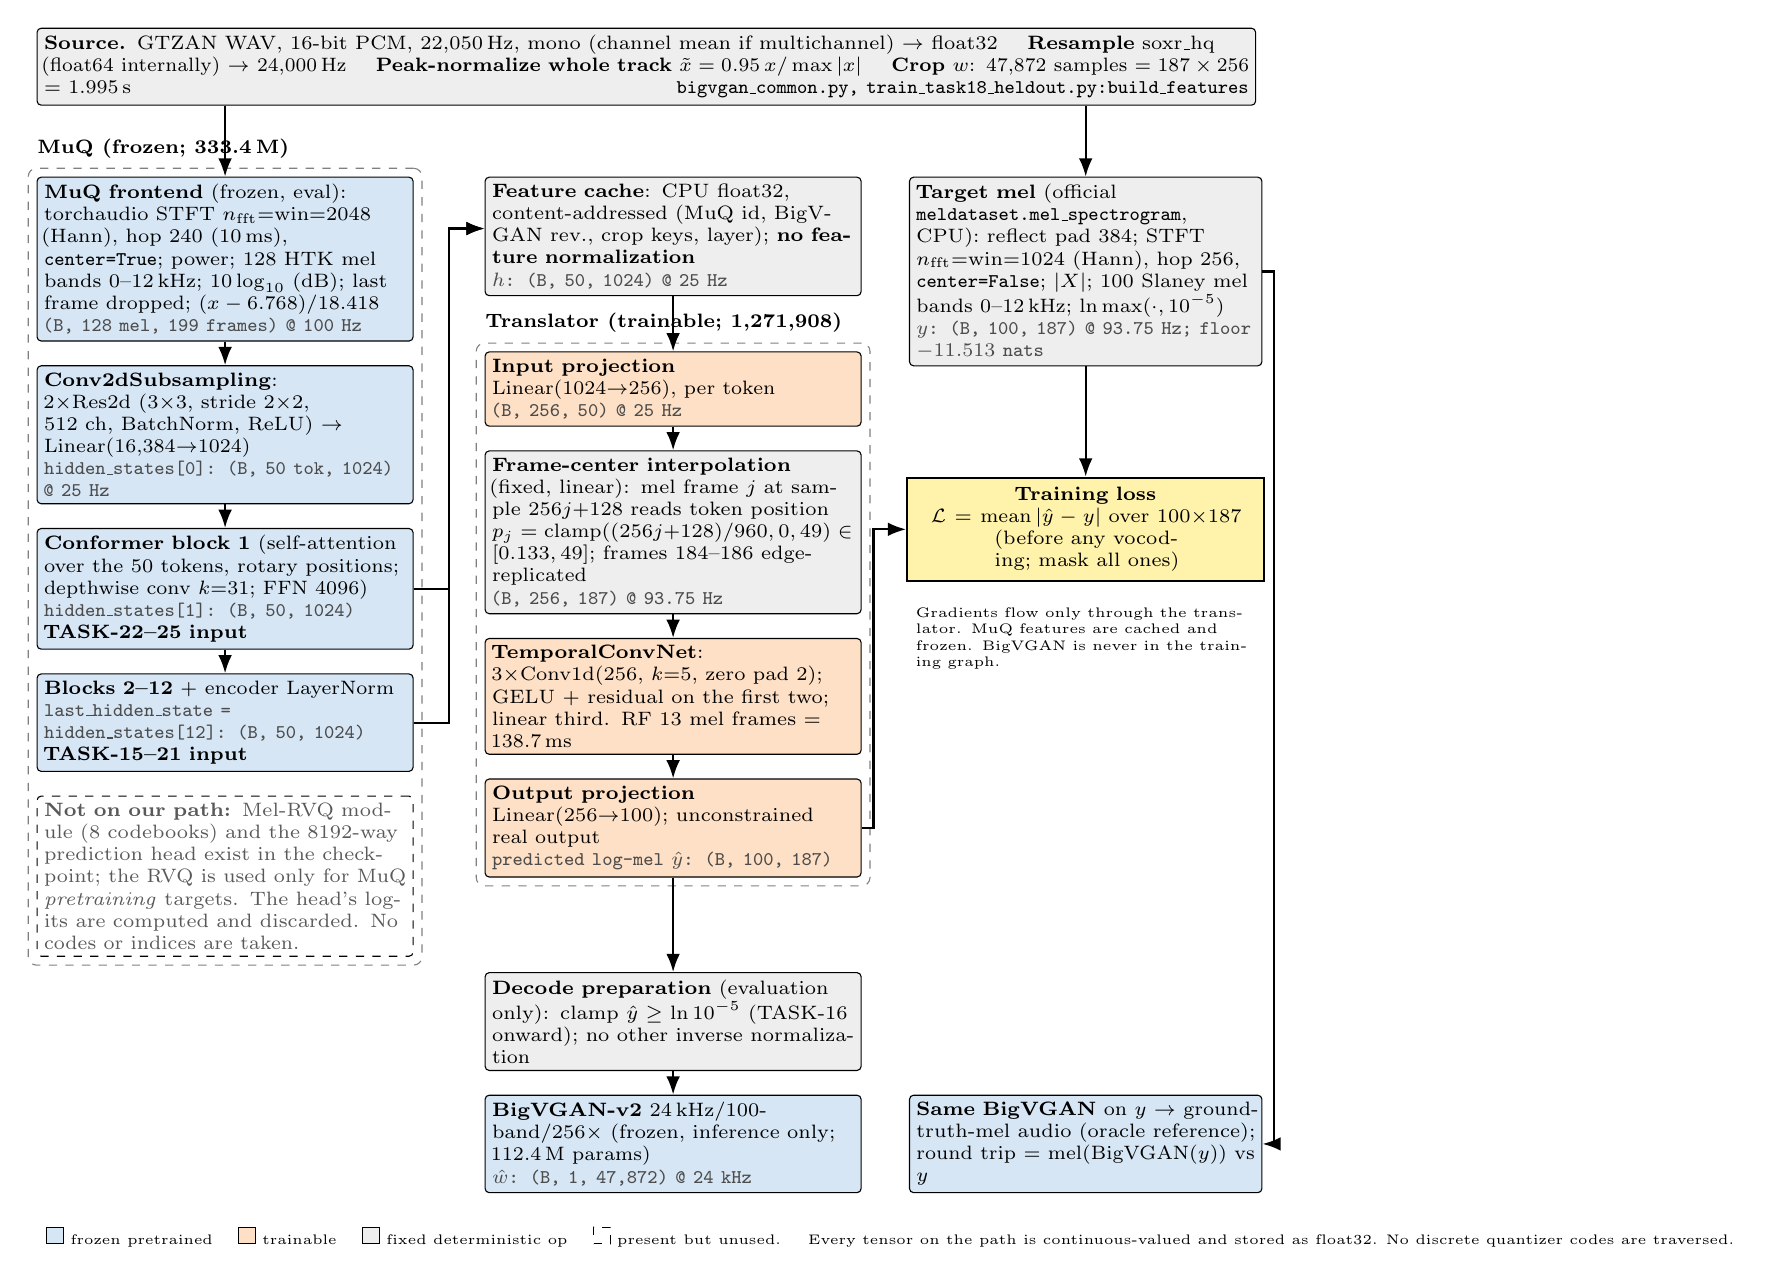
\begin{tikzpicture}[
  font=\scriptsize, >=Latex, node distance=3mm,
  box/.style={draw, rounded corners=1.5pt, align=left, inner sep=2.5pt, text width=#1},
  box/.default=4.6cm,
  det/.style={box=#1, fill=detcol},
  frz/.style={box=#1, fill=frzcol},
  trn/.style={box=#1, fill=trncol},
  det/.default=4.6cm, frz/.default=4.6cm, trn/.default=4.6cm,
  unused/.style={draw, dashed, rounded corners=1.5pt, align=left, inner sep=2.5pt, text width=4.6cm, text=black!65},
  shape/.style={font=\scriptsize\ttfamily, text=black!75},
  arr/.style={->, thick},
  grp/.style={draw=black!50, dashed, rounded corners=3pt, inner sep=3pt},
]
% ---------------- shared front end
\node[det=15.3cm] (src) {\textbf{Source.} GTZAN WAV, 16-bit PCM, 22{,}050\,Hz, mono (channel mean if multichannel) $\to$ float32 \quad
  \textbf{Resample} soxr\_hq (float64 internally) $\to$ 24{,}000\,Hz \quad
  \textbf{Peak-normalize whole track} $\tilde x = 0.95\,x/\max|x|$ \quad
  \textbf{Crop} $w$: 47{,}872 samples $=187\times256$ = 1.995\,s \hfill \texttt{bigvgan\_common.py, train\_task18\_heldout.py:build\_features}};
% ---------------- MuQ column
\node[frz, below=9mm of src.south west, anchor=north west] (fe) {\textbf{MuQ frontend} (frozen, eval): torchaudio STFT $n_\mathrm{fft}{=}$win${=}2048$ (Hann), hop 240 (10\,ms), \texttt{center=True}; power; 128 HTK mel bands 0--12\,kHz; $10\log_{10}$ (dB); last frame dropped; $(x-6.768)/18.418$\\
  \textcolor{black!70}{\ttfamily (B, 128 mel, 199 frames) @ 100 Hz}};
\node[frz, below=of fe] (conv) {\textbf{Conv2dSubsampling}: 2$\times$Res2d (3$\times$3, stride 2$\times$2, 512 ch, BatchNorm, ReLU) $\to$ Linear(16{,}384$\to$1024)\\
  \textcolor{black!70}{\ttfamily hidden\_states[0]: (B, 50 tok, 1024) @ 25 Hz}};
\node[frz, below=of conv] (b1) {\textbf{Conformer block 1} (self-attention over the 50 tokens, rotary positions; depthwise conv $k{=}31$; FFN 4096)\\
  \textcolor{black!70}{\ttfamily hidden\_states[1]: (B, 50, 1024)} \hfill\textbf{TASK-22--25 input}};
\node[frz, below=of b1] (b12) {\textbf{Blocks 2--12} + encoder LayerNorm\\
  \textcolor{black!70}{\ttfamily last\_hidden\_state = hidden\_states[12]: (B, 50, 1024)} \hfill\textbf{TASK-15--21 input}};
\node[unused, below=of b12] (rvq) {\textbf{Not on our path:} Mel-RVQ module (8 codebooks) and the 8192-way prediction head exist in the checkpoint; the RVQ is used only for MuQ \emph{pretraining} targets. The head's logits are computed and discarded. No codes or indices are taken.};
\node[grp, fit=(fe)(conv)(b1)(b12)(rvq), label={[font=\scriptsize\bfseries, anchor=south west]north west:MuQ (frozen; 333.4\,M)}] {};
% ---------------- translator column
\node[det, right=9mm of fe.north east, anchor=north west] (cache) {\textbf{Feature cache}: CPU float32, content-addressed (MuQ id, BigVGAN rev., crop keys, layer); \textbf{no feature normalization}\\
  \textcolor{black!70}{\ttfamily $h$: (B, 50, 1024) @ 25 Hz}};
\node[trn, below=7mm of cache] (proj) {\textbf{Input projection} Linear(1024$\to$256), per token\\
  \textcolor{black!70}{\ttfamily (B, 256, 50) @ 25 Hz}};
\node[det, below=of proj] (interp) {\textbf{Frame-center interpolation} (fixed, linear): mel frame $j$ at sample $256j{+}128$ reads token position $p_j=\mathrm{clamp}((256j{+}128)/960,0,49)\in[0.133,49]$; frames 184--186 edge-replicated\\
  \textcolor{black!70}{\ttfamily (B, 256, 187) @ 93.75 Hz}};
\node[trn, below=of interp] (tcn) {\textbf{TemporalConvNet}: 3$\times$Conv1d(256, $k{=}5$, zero pad 2); GELU + residual on the first two; linear third. RF 13 mel frames = 138.7\,ms};
\node[trn, below=of tcn] (out) {\textbf{Output projection} Linear(256$\to$100); unconstrained real output\\
  \textcolor{black!70}{\ttfamily predicted log-mel $\hat y$: (B, 100, 187)}};
\node[grp, fit=(proj)(interp)(tcn)(out), label={[font=\scriptsize\bfseries, anchor=south west]north west:Translator (trainable; 1{,}271{,}908)}] {};
% ---------------- target column
\node[det, right=6mm of cache.north east, anchor=north west, text width=4.3cm] (tmel) {\textbf{Target mel} (official \texttt{meldataset.mel\_spectrogram}, CPU): reflect pad 384; STFT $n_\mathrm{fft}{=}$win${=}1024$ (Hann), hop 256, \texttt{center=False}; $|X|$; 100 Slaney mel bands 0--12\,kHz; $\ln\max(\cdot,10^{-5})$\\
  \textcolor{black!70}{\ttfamily $y$: (B, 100, 187) @ 93.75 Hz; floor $-11.513$ nats}};
\node[draw, thick, fill=losscol, align=center, text width=4.3cm, below=14mm of tmel] (loss) {\textbf{Training loss}\\ $\mathcal L=\mathrm{mean}\,|\hat y-y|$ over $100{\times}187$\\ (before any vocoding; mask all ones)};
% ---------------- decode row
\node[det, below=12mm of out, text width=4.6cm] (clamp) {\textbf{Decode preparation} (evaluation only): clamp $\hat y\ge\ln 10^{-5}$ (TASK-16 onward); no other inverse normalization};
\node[frz, below=of clamp, text width=4.6cm] (vg) {\textbf{BigVGAN-v2} 24\,kHz/100-band/256$\times$ (frozen, inference only; 112.4\,M params)\\
  \textcolor{black!70}{\ttfamily $\hat w$: (B, 1, 47,872) @ 24 kHz}};
\node[frz, right=6mm of vg, text width=4.3cm] (vgo) {\textbf{Same BigVGAN} on $y$ $\to$ ground-truth-mel audio (oracle reference); round trip = $\mathrm{mel}(\mathrm{BigVGAN}(y))$ vs $y$};
% ---------------- arrows
\draw[arr] (src.south -| fe.north) -- (fe.north);
\draw[arr] (src.south -| tmel.north) -- (tmel.north);
\draw[arr] (fe) -- (conv);
\draw[arr] (conv) -- (b1);
\draw[arr] (b1) -- (b12);
\draw[arr] (b1.east) -- ++(4.5mm,0) |- ([yshift=1mm]cache.west);
\draw[arr] (b12.east) -- ++(4.5mm,0) |- ([yshift=1mm]cache.west);
\draw[arr] (cache) -- (proj);
\draw[arr] (proj) -- (interp);
\draw[arr] (interp) -- (tcn);
\draw[arr] (tcn) -- (out);
\draw[arr] (out.east) -- ++(1.5mm,0) |- (loss.west);
\draw[arr] (tmel) -- (loss);
\draw[arr] (out) -- (clamp);
\draw[arr] (clamp) -- (vg);
\draw[arr] (tmel.east) -- ++(1.5mm,0) |- (vgo.east);
\node[font=\tiny, align=left, anchor=north west, text width=4.3cm] at ([yshift=-2mm]loss.south west) {Gradients flow only through the translator. MuQ features are cached and frozen. BigVGAN is never in the training graph.};
% ---------------- legend
\node[anchor=north west, font=\tiny, align=left] at ([yshift=-3mm]vg.south -| rvq.west) {%
  \tikz\node[fill=frzcol,draw,minimum size=6pt,inner sep=0]{}; frozen pretrained \quad
  \tikz\node[fill=trncol,draw,minimum size=6pt,inner sep=0]{}; trainable \quad
  \tikz\node[fill=detcol,draw,minimum size=6pt,inner sep=0]{}; fixed deterministic op \quad
  \tikz\node[draw,dashed,minimum size=6pt,inner sep=0]{}; present but unused. \quad Every tensor on the path is continuous-valued and stored as float32. No discrete quantizer codes are traversed.};
\end{tikzpicture}
}
\caption{\textbf{Implemented pipeline} (schematic layout; operations, shapes and constants from code and from \src{scripts/geometry.json}, measured on the anchor crop). Shapes are for one 1.995\,s crop with batch size $B$. Left: frozen MuQ; middle: trainable translator; right: target branch and the frozen vocoder. The loss (yellow) compares $\hat y$ with $y$ before vocoding.}
\label{fig:pipeline}
\end{figure}

\subsection{Continuous vs discrete, and storage vs mathematics}
\label{sec:discrete}
\begin{itemize}
\item \obs\ \textbf{No discrete bottleneck is traversed.} MuQ's \texttt{forward} calls \texttt{get\_predictions}, which runs \texttt{preprocessing} $\to$ \texttt{normalize} $\to$ \texttt{conv} $\to$ conformer. The checkpoint contains a Mel-RVQ module (\texttt{use\_rvq\_target: true}, 8 codebooks), but it is called only from \texttt{get\_targets}, which builds MuQ's \emph{pretraining} labels. It is never called during feature extraction. A linear head producing 8192 logits is evaluated on the last layer and discarded. No argmax, codebook lookup or index is taken anywhere on our path.
\item MuQ's pretraining predicted discrete Mel-RVQ tokens \citep{zhu2025muq}. That makes the \emph{training objective} discrete-valued; the hidden states are still continuous activations.
\item \textbf{Storage is not continuity.} Every tensor on the path is stored as float32: waveforms, spectrograms, hidden states, cached features, predictions. Float32 is a finite-precision encoding of real values, not a quantizer. The only finite-valued quantities are the 16-bit PCM samples of the source files and integer indices (sample offsets, frame counts). Neither acts as a learned bottleneck.
\item Sample rate is not frame rate. The waveform has 24{,}000 samples/s. MuQ tokens are framed at 25\,Hz (hop 960 samples) and target mel frames at 93.75\,Hz (hop 256). In a $(B,T,C)$ tensor, $T$ counts frames and $C{=}1024$ is the dimension of each frame's vector; the two are independent.
\end{itemize}

\subsection{Representation ledger}
The ledger (Table~\ref{tab:ledger}, landscape, at the end of Section~\ref{sec:models}) lists every stage for the TASK-23 anchor crop, \texttt{rock.00009}, samples 471{,}082--518{,}954 of the 24\,kHz track (19.63--21.62\,s). All shapes were measured by \src{reports/task26_pipeline_report/scripts/inspect_geometry.py} on CPU with the installed models. They match the cached TASK-22/23 tensors: the recomputed target mel differs from the cache by at most $3.0{\times}10^{-4}$ nats; recomputed block-1 features have relative RMS difference $5.0{\times}10^{-4}$ from the ACES-built cache.

\paragraph{Nominal rate vs finite-crop count.}
\begin{itemize}
\item \textbf{MuQ.} Its STFT (\texttt{center=True}) gives $\lfloor 47872/240\rfloor+1=200$ frames, and MuQ drops the last one: 199. Two stride-2 convolutions with padding 1 give $\lceil 199/2\rceil=100$, then 50 tokens. The notes' ``25.07 fps'' is $50/1.9947$\,s, a finite-crop count. The nominal rate is 25\,Hz: token $i$ is centered at sample $960i$, so the last token center (47{,}040) is 832 samples before the crop end.
\item \textbf{Target mel.} It is padded by $(1024-256)/2=384$ samples on each side with \texttt{center=False}: $(47872+768-1024)/256+1=187$ frames. The crop length was chosen as $187\times256$, so mel frames, BigVGAN output (256$\times$ upsampling) and the original crop all have identical lengths with no trimming.
\end{itemize}


% =====================================================================================================
\section{Models and alignment}
\label{sec:models}

\subsection{MuQ}
\begin{itemize}
\item \textbf{Checkpoint.} \texttt{OpenMuQ/MuQ-large-msd-iter} (Hugging Face snapshot \texttt{0562a578\ldots}), loaded by \texttt{muq 0.1.0} with \texttt{transformers 4.55.0}.
\item \textbf{Architecture.} 12 conformer layers, width 1024 (\texttt{encoder\_depth: 12} overrides the \texttt{num\_hidden\_layers: 24} left in its \texttt{w2v2\_config}). \texttt{is\_flash: false}. In eval mode dropout is inactive and BatchNorm uses stored statistics.
\item \textbf{Frontend and downsampling.} 128-band power mel at 100\,Hz, in dB, globally standardized. The Conv2d subsampling reduces time by 4 (to 25\,Hz) and frequency by 4. A Linear maps the $512\times32$ map to 1024 channels.
\item \textbf{``First block''.} \texttt{transformers}' \texttt{Wav2Vec2ConformerEncoder} appends a hidden state \emph{before} each layer, then appends the LayerNorm of the last layer's output:
  \begin{itemize}
  \item \texttt{hidden\_states[0]} is the frontend output (the input to block~1).
  \item \texttt{hidden\_states[$k$]} is the output of block $k$, for $k=1..11$.
  \item \texttt{hidden\_states[12]} is LayerNorm(block 12) $=$ \texttt{last\_hidden\_state}.
  \end{itemize}
  ``First block'' means \texttt{hidden\_states[1]}. Forward hooks check this on every extraction batch (800 batches in the TASK-22 cache; re-checked in \src{geometry.json}).
\item \textbf{Block 1 vs last layer.} The two have the same shape and token grid, but differ in scale (std 1.72 vs 0.90 on the anchor) and in content (mean per-frame cosine 0.097 between them on the anchor; 0.11 in the TASK-22 notes).
\item \textbf{Context.} Features are extracted from each \emph{isolated} 1.995\,s crop, not from the full track. Through self-attention, every token, including block~1's, depends on all of the crop and on nothing outside it.
\end{itemize}

\subsection{Translator}
\begin{itemize}
\item \textbf{Architecture.} \texttt{MuQToMelTranslator(1024, hidden=256, 100)}:
  \begin{itemize}
  \item Linear(1024$\to$256): 262{,}400 parameters.
  \item Fixed frame-center interpolation.
  \item TemporalConvNet: three Conv1d(256, 256, $k{=}5$), GELU and residual on the first two (983{,}808 parameters).
  \item Linear(256$\to$100): 25{,}700 parameters.
  \end{itemize}
  Total 1{,}271{,}908; about 202\,M MACs per crop.
\item \textbf{Output.} Unconstrained real log-mel; no activation and no clamp in training. The floor clamp is applied only before BigVGAN.
\item \textbf{Receptive field.} 13 frames of the \emph{mel} grid (138.7\,ms). Projected onto MuQ tokens through the 2-tap interpolation, an output frame is influenced by 2--6 tokens (median 5), i.e.\ 80--240\,ms of token grid. Because each token already carries crop-wide context, the translator's receptive field does \emph{not} bound the audio context an output frame depends on.
\item \textbf{TASK-25 arm E (width $\times$2).} Hidden 512, same depth, kernels, receptive field, activations and interpolation: 4{,}509{,}796 parameters, 771\,M MACs. Fresh seed-0 initialization.
\item \textbf{TASK-25 arm F (learned resampler).}
  \begin{itemize}
  \item Replaces the 2-tap interpolation with a 4-tap local resampler over taps $\{-1,0,1,2\}$ around $\lfloor p_j\rfloor$.
  \item Weights are $[0,1{-}w,w,0]+\delta(w)$, where $\delta$ is an MLP $1\to32\to4\cdot256$ of the phase $w$, per channel.
  \item The MLP's output layer is initialized at zero, so F starts bit-identical to the current decoder.
  \item Edge taps are clamped. Cost: +33{,}856 parameters (+2.7\%); influence per output frame 3--8 tokens (median 7).
  \end{itemize}
\end{itemize}

\subsection{BigVGAN}
\begin{itemize}
\item \textbf{Checkpoint.} \texttt{nvidia/bigvgan\_v2\_24khz\_100band\_256x} at revision \texttt{c329ede9\ldots}, generator sha256 \texttt{6f9c5715\ldots}. Code and checkpoint come from the Hugging Face repository itself (\src{scripts/fetch_bigvgan.py}). It is loaded with \texttt{from\_pretrained(use\_cuda\_kernel=False)} and \texttt{remove\_weight\_norm()}, and all parameters have \texttt{requires\_grad=False}.
\item \textbf{Mel convention.} The model expects exactly the target mel convention of Table~\ref{tab:ledger}: 24\,kHz, 100 bands, $n_\mathrm{fft}{=}1024$, hop 256, $f_\mathrm{max}$ = Nyquist, $\ln$ with clip $10^{-5}$.
\item \textbf{Volume.} Its training path peak-normalizes waveforms to 0.95; we reproduce this per track.
\item \textbf{Role.} BigVGAN is run only at evaluation, in inference mode. No gradient ever passes through it, and the training loss is applied before vocoding in every task.
\end{itemize}

\subsection{Alignment: what is assumed and what has been checked}
\begin{figure}[t]
\centering
\resizebox{\textwidth}{!}{% Figure B: temporal grids at the start and end of one 47,872-sample crop. Drawn to scale: x is in samples of
% the 24 kHz crop, relative to each panel's first sample (TeX dimensions cannot hold 47,872 directly, so
% integer arithmetic uses \numexpr). Centers follow time_alignment.py (verified in scripts/geometry.json):
% MuQ frontend frame k at 240k (center=True; frame 199 dropped by MuQ), token i at 960i, mel frame j at 256j+128.
\newcommand{\gridpanel}[3]{% #1 first sample (int), #2 y offset, #3 title
\begin{scope}[yshift=#2cm, x=0.0045cm]
  \def\A{#1}
  \node[anchor=south west, font=\scriptsize\bfseries] at (0,3.45) {#3};
  \edef\cs{\the\numexpr 0-\A\relax}\ifnum\cs<0 \def\cs{0}\fi
  \edef\ce{\the\numexpr 47872-\A\relax}\ifnum\ce>3000 \def\ce{3000}\fi
  \fill[black!6] (\cs,0.05) rectangle (\ce,3.3);
  \draw[->] (0,3.0) -- (3050,3.0);
  \foreach \s in {0,...,100}{\edef\c{\the\numexpr 480*\s-\A\relax}
     \ifnum\c<0\else\ifnum\c>3000\else \draw (\c,2.93) -- (\c,3.07);\fi\fi}
  \foreach \k in {0,...,199}{\edef\c{\the\numexpr 240*\k-\A\relax}
     \ifnum\c<0\else\ifnum\c>3000\else
       \ifnum\k<199 \fill[muqcol!60] (\c,2.25) circle (1pt);\else \draw[muqcol!60] (\c,2.25) circle (1.3pt) node[above, font=\tiny] {dropped};\fi\fi\fi}
  \foreach \i in {0,...,49}{\edef\c{\the\numexpr 960*\i-\A\relax}
     \ifnum\c<0\else\ifnum\c>3000\else
       \draw[muqcol, very thick] (\c,1.3) -- (\c,1.6); \node[font=\tiny, muqcol, anchor=south] at (\c,1.6) {$i{=}\i$};\fi\fi}
  \foreach \j in {0,...,186}{\edef\c{\the\numexpr 256*\j+128-\A\relax}
     \ifnum\c<0\else\ifnum\c>3000\else \fill[melcol] (\c,0.6) circle (1.2pt);\fi\fi}
  \foreach \y/\t in {3.0/{waveform 24 kHz (ticks: 480 samples = 20 ms)},
                     2.25/{MuQ STFT frames, hop 240 = 10 ms (100 Hz)},
                     1.45/{MuQ tokens, hop 960 = 40 ms (25 Hz)},
                     0.6/{BigVGAN mel frames, hop 256 = 10.67 ms (93.75 Hz)}}
     \node[anchor=east, align=right, font=\tiny, text width=2.6cm] at (-30,\y) {\t};
\end{scope}}
\begin{tikzpicture}[font=\scriptsize, >=Latex]
  \gridpanel{-500}{0}{(a) Crop start: samples $-500$ to 2{,}500}
  \gridpanel{45200}{-4.4}{(b) Crop end: samples 45{,}200 to 48{,}200}
  % panel (a) annotations, x relative to sample -500
  \begin{scope}[x=0.0045cm]
    \draw[melcol, |-|] (116,0.25) -- (1140,0.25) node[pos=0.5, below, font=\tiny, text=melcol] {mel frame 0 window: samples $-384$..640 (reflect-padded outside the crop)};
    \draw[melcol, densely dotted, thick] (628,0.6) -- (628,1.3);
    \node[font=\tiny, melcol, anchor=west] at (640,0.95) {$p_0 = 128/960 = 0.133$ (frame 0 reads mostly token 0)};
    \draw[muqcol!70, |-|] (0,2.5) -- (1524,2.5);
    \node[font=\tiny, muqcol!80, anchor=west] at (1540,2.5) {STFT frame 0 window: samples $-1024$..1024};
    \node[font=\tiny, anchor=north] at (500,0.05) {crop start (sample 0)};
  \end{scope}
  % panel (b) annotations, x relative to sample 45,200
  \begin{scope}[yshift=-4.4cm, x=0.0045cm]
    \draw[thick] (2672,0.0) -- (2672,3.35) node[above, font=\tiny] {crop end (47{,}872)};
    \draw[melcol, densely dotted, thick] (1840,1.3) -- (1840,0.35);
    \node[font=\tiny, align=left, anchor=north west, text=melcol] at (30,0.4) {mel frames 184--186 (centers 47{,}232; 47{,}488; 47{,}744) lie after the last token center (47{,}040, $i{=}49$):\\their source positions are clamped to $p{=}49$ (edge replication).};
  \end{scope}
\end{tikzpicture}
}
\caption{\textbf{Temporal grids} of the waveform, MuQ frontend frames, MuQ tokens and target-mel frames at the start and end of a crop, drawn to scale from the implemented center formulas. Mel frame $j$ reads MuQ position $p_j=(256j+128)/960$. The last three mel frames lie after the last token center and are edge-replicated. A token's ``center'' is the geometric center of the convolutional frontend; after conformer self-attention every token depends on the whole crop, so the center is a convention, not a measured localization. Shaded: inside the crop. The finite crop yields 50 tokens / 1.995\,s = 25.07 tokens/s; the nominal rate is 25\,Hz.}
\label{fig:timegrid}
\end{figure}

\begin{itemize}
\item \textbf{Assumed.} Token $i$ ``represents'' time $960i$: the geometric center of the frontend's convolutions, given \texttt{center=True} STFT frames at $240k$ (Fig.~\ref{fig:timegrid}). Mel frame $j$ represents $256j+128$. After the conformer, every token mixes the whole crop, so ``token time'' is a convention, not a measured localization.
\item \textbf{Checked.}
  \begin{itemize}
  \item TASK-16 derived both center sets from the loaded models and verified the mel centers against impulse responses of the official function. TASK-15's \texttt{F.interpolate(align\_corners=False)} had placed token $i$ at $(i+\tfrac12)$ hops, about 15--20\,ms early; correcting it did not materially change the $N{=}2$ result.
  \item Decoded audio and the original crop line up closely: the best-correlation lag between BigVGAN output and the original was 32 samples (1.3\,ms) on \texttt{pop.00012} (TASK-16). This concerns the vocoder path, not the MuQ-to-mel mapping.
  \item Every model beats the \emph{shuffled-in-time} control by a wide margin (TASK-22 block 1: $\Delta=0.52$--0.57 nats). The translator therefore uses temporal order, and coarse timing is right.
  \end{itemize}
\item \textbf{Not checked.} No experiment has varied the alignment offset to see whether $\pm$5--20\,ms shifts lower the error. The effect of isolated-crop context on MuQ's edge tokens, versus extraction with surrounding track context, has not been measured. Matching tensor lengths (187 = 187) is not, by itself, evidence of timestamp alignment.
\end{itemize}

\begin{landscape}
\footnotesize
\setlength{\tabcolsep}{2.5pt}
\begin{longtable}{L{2.5cm}L{0.6cm}L{2.9cm}L{1.9cm}L{3.8cm}L{1.8cm}L{3.0cm}L{1.75cm}L{3.3cm}}
\caption{\textbf{Representation ledger} for one crop (anchor \texttt{rock.00009}, 1.995\,s). Axes: B batch, T time (samples or frames), F mel bins, C channels. ``Value'': continuous (real-valued) or discrete. All arrays are float32 unless stated.}\label{tab:ledger}\\
\toprule
Stage / module & Sym. & Layout; anchor shape & Rate; hop & Transform parameters & Value; dtype & Scaling; units; clipping & Status & Context; padding; boundary\\
\midrule\endfirsthead
\toprule
Stage / module & Sym. & Layout; anchor shape & Rate; hop & Transform parameters & Value; dtype & Scaling; units; clipping & Status & Context; padding; boundary\\
\midrule\endhead
\bottomrule\endfoot
GTZAN source file & $x_\mathrm{raw}$ & (T) 661{,}794 & 22{,}050\,Hz & \texttt{soundfile} read; channel mean if multichannel (GTZAN is mono) & 16-bit PCM $\to$ float32 & $[-1,1]$; anchor source peaks at full scale (alternating $\pm1$ at 7.18\,s) & data & whole track\\
Resampled track & $x$ & (T) 720{,}321 & 24{,}000\,Hz & \texttt{librosa.resample}, \texttt{soxr\_hq} (float64 internally); NaN/Inf/silence/clipping checks & cont.; float32 & no clipping; anchor peak 1.992 (overshoot of the source glitch) & deterministic & whole track\\
Peak-normalized track & $\tilde x$ & (T) 720{,}321 & 24\,kHz & $0.95\,x/\max|x|$ (\texttt{librosa.util.normalize}) & cont.; float32 & gain set by whole-track peak (anchor: $\times0.477$) & deterministic & whole track; one outlier sets gain\\
Crop (shared by both branches) & $w$ & (B, T) (1, 47{,}872) & 24\,kHz & start sample from manifest (471{,}082); length $187\times256$ & cont.; float32 & peak 0.477, RMS 0.088 & deterministic & \textbf{isolated crop}: no audio outside it is seen downstream\\
\midrule
\multicolumn{9}{l}{\textit{MuQ branch (frozen; \texttt{OpenMuQ/MuQ-large-msd-iter}, eval mode, \texttt{inference\_mode}; 333{,}401{,}472 parameters, none trainable)}}\\
MuQ log-mel frontend & $S$ & (B, F, T) (1, 128, 199) & 100\,Hz; 240 (10\,ms) & torchaudio \texttt{MelSpectrogram}: $n_\mathrm{fft}{=}$win${=}2048$ Hann, hop 240, \texttt{center=True} (reflect), power 2, 128 HTK mel bands 0--12\,kHz, no filter norm; \texttt{AmplitudeToDB} ($10\log_{10}$, no top\_db); last frame dropped & cont.; float32 & dB & frozen (fixed) & reflect pad 1024 at crop edges\\
MuQ input normalization & $\bar S$ & (1, 128, 199) & 100\,Hz & $(S-6.7684)/18.4179$ (global stats in the checkpoint) & cont.; float32 & dimensionless; anchor mean $-0.77$, std 1.30 & frozen & frame-local\\
Conv2dSubsampling & $h_0$ & (B, T, C) (1, 50, 1024) & 25\,Hz; 960 (40\,ms) & 2$\times$Res2dModule (Conv2d 3$\times$3, stride 2$\times$2, pad 1, 512 ch, BatchNorm in eval mode, ReLU, conv shortcut): F $128{\to}32$, T $199{\to}50$; flatten $512{\cdot}32{=}16384$; Linear$\to$1024 & cont.; float32 & --- & frozen & conv zero-padding; token $i$ center at sample $960i$ (geometric)\\
Conformer block 1 output & $h_1$ & (1, 50, 1024) & 25\,Hz & Wav2Vec2-Conformer layer: FFN(4096) / 16-head self-attention with rotary positions / depthwise conv $k{=}31$ / FFN; swish; \texttt{hidden\_states[1]}, hook-verified to equal \texttt{layers[0]} output & cont.; float32 & anchor std 1.72 & frozen & \textbf{all 50 tokens} via attention (crop-wide)\\
Last hidden state & $h_{12}$ & (1, 50, 1024) & 25\,Hz & blocks 2--12, then encoder LayerNorm; \texttt{hidden\_states[12]} = \texttt{last\_hidden\_state} & cont.; float32 & anchor std 0.90 & frozen & crop-wide\\
(Unused) RVQ and prediction head & --- & --- & --- & Mel-RVQ (8 codebooks) for pretraining labels; Linear(1024$\to$8192) logits computed and discarded & would be discrete; not used & --- & present, unused & ---\\
Feature cache & $h$ & (N, 50, 1024) & 25\,Hz & content-addressed \texttt{torch.save}; layer-keyed (TASK-22+); extracted in batches of 16 crops & cont.; float32 (CPU) & \textbf{no normalization} & stored & per isolated crop\\
\midrule
\multicolumn{9}{l}{\textit{Translator (trainable; \texttt{MuQToMelTranslator}, 1{,}271{,}908 parameters, FP32, Adam)}}\\
Input projection & $u$ & (B, C, T) (1, 256, 50) & 25\,Hz & Linear(1024$\to$256), per token & cont.; float32 & --- & trainable & none (pointwise)\\
Frame-center interpolation & $v$ & (1, 256, 187) & 93.75\,Hz; 256 & $v_j=(1{-}w_j)u_{\lfloor p_j\rfloor}+w_j u_{\lfloor p_j\rfloor+1}$, $p_j=\mathrm{clamp}((256j{+}128)/960,0,49)$; 3.75 mel frames per token, 15 phase values & cont.; float32 & --- & fixed & 2 tokens per frame; frames 184--186 edge-replicated ($p{=}49$)\\
TemporalConvNet & $g$ & (1, 187, 256) & 93.75\,Hz & 3$\times$Conv1d(256$\to$256, $k{=}5$, pad 2); $x{+}\mathrm{GELU}(\cdot)$ twice, linear third & cont.; float32 & --- & trainable & RF 13 frames = 138.7\,ms; zero padding within 6 frames of either edge\\
Output projection & $\hat y$ & (B, F, T) (1, 100, 187) & 93.75\,Hz & Linear(256$\to$100) & cont.; float32 & natural-log magnitude (nats); \textbf{unconstrained} & trainable & per frame\\
\midrule
\multicolumn{9}{l}{\textit{Target branch and loss}}\\
Target mel (official BigVGAN code) & $y$ & (B, F, T) (1, 100, 187) & 93.75\,Hz; 256 (10.67\,ms) & reflect pad 384; \texttt{torch.stft} $n_\mathrm{fft}{=}$win${=}1024$ Hann, hop 256, \texttt{center=False}; $\sqrt{|X|^2{+}10^{-9}}$; 100 Slaney-normalized mel bands (librosa), 0--12\,kHz; $\ln\max(\cdot,10^{-5})$; computed on CPU & cont.; float32 & nats; floor $-11.513$; anchor range $[-11.513,0.449]$, 805/18{,}700 bins at floor & deterministic & frame $j$ centered at $256j{+}128$; windows of frames 0--1 and 185--186 extend into reflect padding\\
Training loss & $\mathcal L$ & scalar & --- & $\mathrm{mean}|\hat y-y|$ over B$\times$100$\times$187 (TASK-23+: masked form; mask all ones) & cont.; float32 & nats & --- & every frame weighted equally\\
\midrule
\multicolumn{9}{l}{\textit{Decoding (evaluation only; never in the training graph)}}\\
Decode preparation & $\hat y_c$ & (1, 100, 187) & 93.75\,Hz & $\max(\hat y,\ln10^{-5})$ (TASK-16+; TASK-15 unclamped); no other inverse transform & cont.; float32 & nats & deterministic & ---\\
BigVGAN-v2 generator & $\hat w$ & (B, 1, T) (1, 1, 47{,}872) & 24\,kHz & upsampling $4{\cdot}4{\cdot}2{\cdot}2{\cdot}2{\cdot}2=256$; Snake-Beta activations; weight norm removed; \texttt{use\_cuda\_kernel=False} & cont.; float32 & waveform (no clipping applied) & frozen (112{,}414{,}512 params) & convolutional context over the 187-frame input\\
Oracle reference & $w_\mathrm{GT}$ & (1, 1, 47{,}872) & 24\,kHz & BigVGAN$(y)$; round trip $=\mathrm{mean}|\mathrm{mel}(w_\mathrm{GT})-y|$ & cont.; float32 & nats & frozen & ---\\
\end{longtable}
\end{landscape}

% =====================================================================================================
\section{How results are measured}
\label{sec:metrics}
\begin{itemize}
\item \textbf{Direct pre-vocoder mel L1.} $\mathrm{mean}|\hat y-y|$ in nats over all bins and frames, before clamping. This is the loss, and the main metric in every task.
\item \textbf{Round trip.} $\mathrm{mean}|\mathrm{mel}(\mathrm{BigVGAN}(y))-y|$, about 0.11 on every set. It measures how far BigVGAN's \emph{audio} drifts from the true mel when re-analysed, which is a different quantity. It is not a lower bound on direct L1 (TASK-15 reached 0.024), and the ground-truth-mel audio is a reference, not an upper bound on every possible method. Ratios such as ``held-out error is 4.3$\times$ the round trip'' in the notes compare two different quantities and serve only for orientation.
\item \textbf{Resynthesis metrics.} Mel L1 and multi-resolution STFT distance between decoded and original audio, reported in TASK-15/16/18. Waveform correlation depends on phase: mel vocoding does not preserve phase, and the oracle itself reaches only $\approx$0.14 against the original.
\item \textbf{Evaluation regimes.}
  \begin{itemize}
  \item \emph{Training crops} (``memorized'', or the fixed pools of TASK-23--25).
  \item \emph{Unseen crops of training tracks} (``train\_unseen'').
  \item \emph{Unseen tracks}: val/test from TASK-18; val2/test2 from TASK-19, 24 tracks each.
  \item \emph{Monitoring crops} (TASK-24/25): 16 crops from 16 GTZAN-train tracks not in the 256-crop pool. They are unseen by those decoders, but they are a reused diagnostic set, not a held-out confirmation set.
  \end{itemize}
\item \textbf{Checkpoints.} TASK-18--22 select ``best'' on primary val mel L1 only; val is therefore optimistically biased. TASK-21 selected among 22{,}297 checks. Test, val2 and test2 were never used for decisions, but all four sets have been evaluated in several tasks. They are reused evaluation sets, not untouched confirmation data; none remains. TASK-23--25 select on training error, and their primary comparisons use final checkpoints.
\item \textbf{Matching.} \emph{Steps} or \emph{updates} count optimizer updates (TASK-22 vs 21 at matched steps). \emph{Presentations} count crop exposures (TASK-25 matches 819{,}200 per arm, so batch-1 arms take 16$\times$ more updates). \emph{Compute} (MACs, wall time) was never matched.
\item \textbf{Uncertainty.} The bootstrap CIs (track-clustered in TASK-18--22; over crops in TASK-25) describe sampling of \emph{evaluation} crops and tracks for one trained model. Every task trained one seed, so variability across training seeds is unmeasured. TASK-23's same-initialization repeat (B vs C) shows that MPS/XPU nondeterminism alone can produce spikes of order 1 nat.
\end{itemize}

% =====================================================================================================
\section{The experiment sequence}
\label{sec:sequence}
\begin{figure}[t]
\centering
\resizebox{\textwidth}{!}{% Figure C: experiment sequence of the MuQ -> mel -> BigVGAN line (schematic).
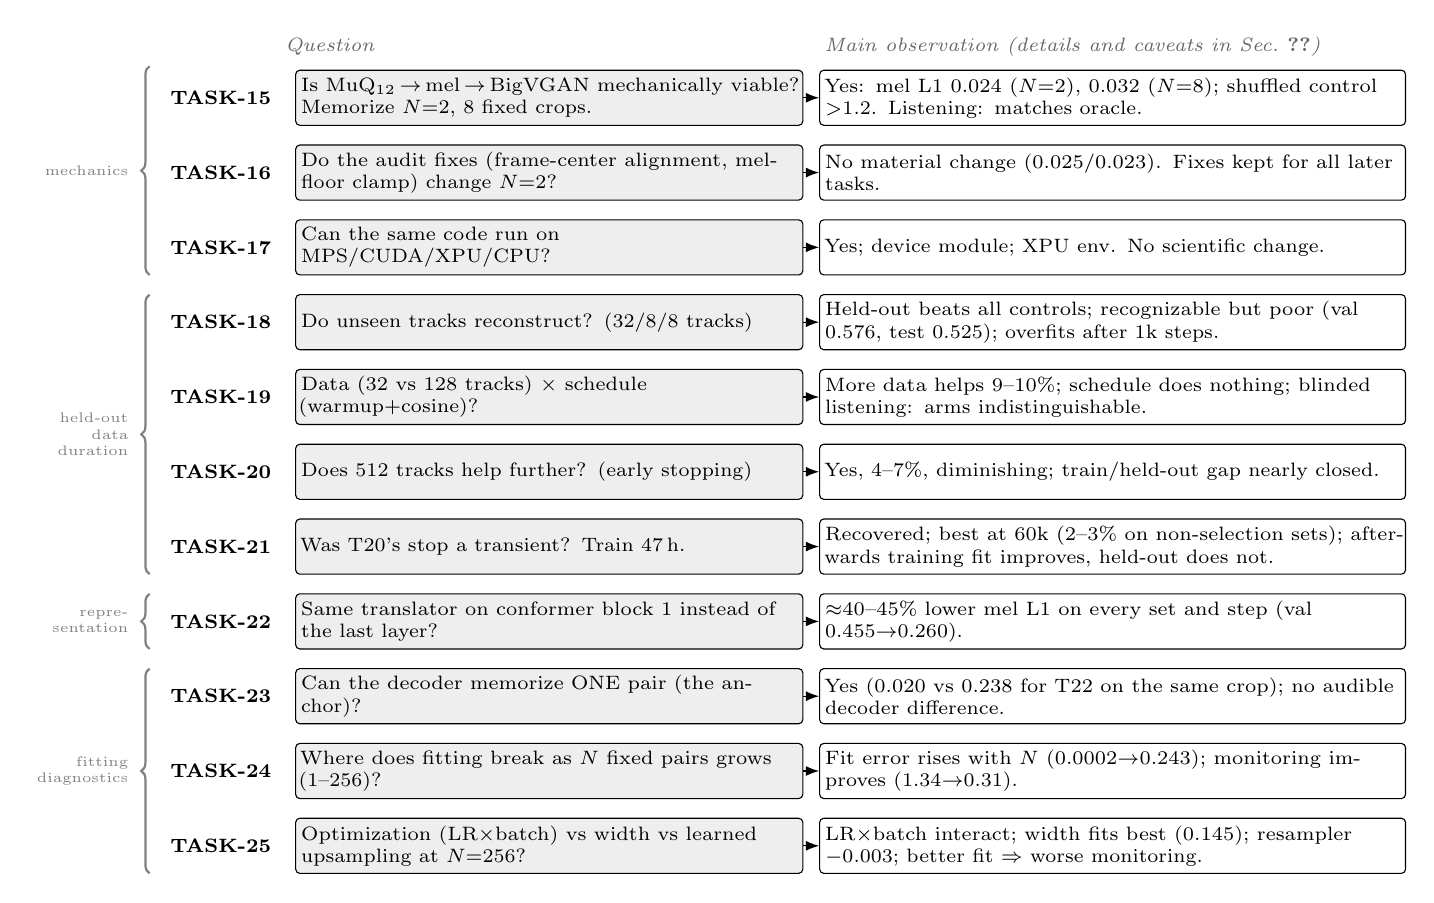
\begin{tikzpicture}[font=\scriptsize, >=Latex,
  q/.style={draw, rounded corners=1.5pt, fill=detcol, text width=6.3cm, align=left, inner sep=2pt, minimum height=7mm},
  a/.style={draw, rounded corners=1.5pt, fill=white, text width=7.3cm, align=left, inner sep=2pt, minimum height=7mm},
  t/.style={font=\scriptsize\bfseries, text width=1.35cm, align=left, anchor=west},
  ph/.style={font=\scriptsize\itshape, text=black!60, anchor=west}]
\def\rows{%
  15/{Is MuQ$_{12}$\,$\to$\,mel\,$\to$\,BigVGAN mechanically viable? Memorize $N{=}2$, 8 fixed crops.}/{Yes: mel L1 0.024 ($N{=}2$), 0.032 ($N{=}8$); shuffled control $>$1.2. Listening: matches oracle.},
  16/{Do the audit fixes (frame-center alignment, mel-floor clamp) change $N{=}2$?}/{No material change (0.025/0.023). Fixes kept for all later tasks.},
  17/{Can the same code run on MPS/CUDA/XPU/CPU?}/{Yes; device module; XPU env. No scientific change.},
  18/{Do unseen tracks reconstruct? (32/8/8 tracks)}/{Held-out beats all controls; recognizable but poor (val 0.576, test 0.525); overfits after 1k steps.},
  19/{Data (32 vs 128 tracks) $\times$ schedule (warmup+cosine)?}/{More data helps 9--10\%; schedule does nothing; blinded listening: arms indistinguishable.},
  20/{Does 512 tracks help further? (early stopping)}/{Yes, 4--7\%, diminishing; train/held-out gap nearly closed.},
  21/{Was T20's stop a transient? Train 47\,h.}/{Recovered; best at 60k (2--3\% on non-selection sets); afterwards training fit improves, held-out does not.},
  22/{Same translator on conformer block 1 instead of the last layer?}/{$\approx$40--45\% lower mel L1 on every set and step (val 0.455$\to$0.260).},
  23/{Can the decoder memorize ONE pair (the anchor)?}/{Yes (0.020 vs 0.238 for T22 on the same crop); no audible decoder difference.},
  24/{Where does fitting break as $N$ fixed pairs grows (1--256)?}/{Fit error rises with $N$ (0.0002$\to$0.243); monitoring improves (1.34$\to$0.31).},
  25/{Optimization (LR$\times$batch) vs width vs learned upsampling at $N{=}256$?}/{LR$\times$batch interact; width fits best (0.145); resampler $-$0.003; better fit $\Rightarrow$ worse monitoring.}}
\foreach \n/\qq/\aa [count=\r] in \rows {
  \node[t] (t\r) at (0,-\r*0.95) {TASK-\n};
  \node[q, right=1mm of t\r] (q\r) {\qq};
  \node[a, right=2mm of q\r] (a\r) {\aa};
  \draw[->] (q\r) -- (a\r);
}
\node[ph] at (1.45,-0.3) {Question};
\node[ph] at (8.3,-0.3) {Main observation (details and caveats in Sec.~\ref{sec:sequence})};
\draw[decorate, decoration={brace, amplitude=3pt, mirror}, thick, black!50] (-0.15,-0.55) -- node[left=4pt, align=right, font=\tiny] {mechanics} (-0.15,-3.2);
\draw[decorate, decoration={brace, amplitude=3pt, mirror}, thick, black!50] (-0.15,-3.45) -- node[left=4pt, align=right, font=\tiny] {held-out\\data\\duration} (-0.15,-7.0);
\draw[decorate, decoration={brace, amplitude=3pt, mirror}, thick, black!50] (-0.15,-7.25) -- node[left=4pt, align=right, font=\tiny] {repre-\\sentation} (-0.15,-7.95);
\draw[decorate, decoration={brace, amplitude=3pt, mirror}, thick, black!50] (-0.15,-8.2) -- node[left=4pt, align=right, font=\tiny] {fitting\\diagnostics} (-0.15,-10.8);
\end{tikzpicture}
}
\caption{\textbf{Experiment sequence} of the BigVGAN line (schematic). Numbers are direct mel L1 in nats; sets and checkpoints differ between rows (see Table~\ref{tab:cross}).}
\label{fig:timeline}
\end{figure}

Every task used frozen MuQ and BigVGAN, the TASK-15 translator (except TASK-25 E/F), raw log-mel targets, L1 loss, Adam (0.9, 0.999) with no weight decay and no gradient clipping, FP32, and seed 0. From TASK-16 on, frame-center alignment and the decode clamp were also standard. Listening was always by one listener (the project lead).

\paragraph{TASK-15 --- mechanical viability.}
\begin{itemize}
\item \textbf{Setup.} $N{=}2$ and $N{=}8$ fixed crops, trained and evaluated on the same crops; \texttt{last\_hidden\_state}; length-resize interpolation; full batch; 5{,}000 steps at LR $10^{-3}$. The best checkpoint by mel L1 was selected on those crops; this protocol change was disclosed after a final-step L1 spike in the first run.
\item \textbf{Results.} $N{=}2$: mel L1 0.024 at step 4{,}750, shuffled-across control 1.20, pred-vs-oracle waveform correlation 0.97. $N{=}8$: 0.032 (correlation 0.92; 6/8 crops pass every pre-registered criterion). The oracle round trip is 0.109.
\item \textbf{Listening.} Unblinded: reconstructions match the oracle at both $N$.
\item \textbf{Supports.} The path is mechanically viable for memorization. It says nothing about generalization.
\end{itemize}

\paragraph{TASK-16 --- audit fixes.}
\begin{itemize}
\item \textbf{Setup.} Frame-center alignment and the decode-time mel-floor clamp, rerun at $N{=}2$.
\item \textbf{Results.} 0.025/0.023 per crop (vs 0.023/0.024 before); the clamp raised 1.5\% and 2.4\% of bins. Listening of the corrected files is pending.
\item \textbf{Supports.} The corrections are immaterial at this scale, and both are kept in all later tasks.
\end{itemize}
\noindent TASK-17 made the code portable (MPS, CUDA, XPU, CPU) without changing the science.

\paragraph{TASK-18 --- held-out tracks.}
\begin{itemize}
\item \textbf{Setup.} 32 training tracks, each with 24 pool crops (768 crops). 8 validation and 8 test tracks, one per genre, with crops at 2, 9, 16 and 23\,s. Checksum-deduplicated split, not artist-aware. Track-balanced batches of 64, 20{,}000 steps at a constant LR of $10^{-3}$; best checkpoint selected on val.
\item \textbf{Results.} Best at step 1{,}000: memorized 0.354, unseen crops of training tracks 0.451, val 0.576, test 0.525. Every control is worse; the closest is shuffled-time at 0.89/0.85. On test, onset correlation is 0.94 and chroma cosine 0.85.
\item \textbf{Listening.} Unblinded: held-out clips are recognizable but poor.
\item \textbf{Supports.} Held-out tracks generalize at a recognizable level. After step 1{,}000 the training error keeps falling while the val error rises, i.e.\ overfitting. The pre-registered code \texttt{UNDERFIT} (memorized error $>2\times$ round trip) is kept as registered.
\end{itemize}

\paragraph{TASK-19 --- data $\times$ schedule.}
\begin{itemize}
\item \textbf{Setup.} 32 vs 128 tracks (the extra 96 checked against the Sturm fault list \citep{sturm2013gtzan}), crossed with recipe A (constant LR) vs B (1k-step warmup to $10^{-3}$, cosine decay to $10^{-5}$); 20k steps each. A secondary held-out set adds 24 + 24 tracks.
\item \textbf{Results.} 128 tracks lower held-out error 8.9\% on the primary set (0.550 $\to$ 0.501, 16/16 tracks) and 10.2\% on the secondary set. Recipe B has no effect. Every arm reaches its val optimum by steps 1{,}000--2{,}500.
\item \textbf{Listening.} \emph{Blinded} (0--4 scale, 16 examples): oracle 4.00; arms 2.69--2.75, indistinguishable from each other; shuffled-time 1.12; shuffled-across and zero 0.00. Two examples were re-rated non-blind after entry errors; conclusions are unchanged without them.
\item \textbf{Supports.} Data helps modestly; the schedule does not. The 9--10\% mel gain is not audible.
\end{itemize}

\paragraph{TASK-20 --- 512 tracks.}
\begin{itemize}
\item \textbf{Setup.} Recipe A with early stopping on val (patience 8 checks of 250 steps); best at step 2{,}250, stopped at 4{,}250.
\item \textbf{Results.} Held-out errors improve 4--7\% over A128: val 0.475, test 0.465, val2 0.481, test2 0.494. Training-crop error gets \emph{worse}: memorized 0.396 $\to$ 0.441. The train/held-out gap nearly closes.
\item \textbf{Listening.} Blinded: A128 = N512 = 2.25, oracle 3.88.
\item \textbf{Supports.} Diminishing returns from data. An Adam/L1 spike at about 3.5k steps fell inside the patience window.
\end{itemize}

\paragraph{TASK-21 --- duration.}
\begin{itemize}
\item \textbf{Setup.} Exact continuation of TASK-20's last checkpoint for 47.0\,h (22.2\,M steps, about 116k passes over the pool), with no early stopping.
\item \textbf{Results.} Best at step 60{,}000: val 0.455 (inflated by selection), test 0.454 ($+2.2\%$, CI touches 0), val2 0.473 ($+1.8\%$, CI includes 0), test2 0.480 ($+2.9\%$). The final checkpoint is about equal to or worse than TASK-20's best on held-out sets, while memorized error keeps falling (0.441 $\to$ 0.391 at best $\to$ 0.368 final).
\item \textbf{Listening.} None.
\item \textbf{Supports.} Longer training recovered from the early transient and helped modestly; after that it increasingly favored training fit over held-out error.
\end{itemize}

\paragraph{TASK-22 --- representation depth.}
\begin{itemize}
\item \textbf{Setup.} The same translator, recipe, seed, sampler and data as TASK-20/21, trained from scratch on \texttt{hidden\_states[1]} for 200k steps and compared at matched steps and window best.
\item \textbf{Results.} Window best: L1 193k vs L12 60k. Held-out errors with block-1 features are 0.257--0.263, against 0.454--0.480 for the last layer ($\Delta$ 0.20--0.22 nats, every CI $>0$, 100\% of tracks). The gain holds at every matched step (36\% at 10k, 44--46\% at 200k). Block-1 memorized and held-out errors are nearly equal (0.255 vs 0.257--0.263). There was one blow-up near step 2{,}000, recovered by about 3{,}000.
\item \textbf{Listening.} A blinded package exists (\src{artifacts/task22/listening_blind_v1/}) but is \textbf{unrated}.
\item \textbf{Supports.} Block-1 features are much more recoverable with \emph{this} decoder and recipe. This does not show that deeper layers discarded information; a different decoder or input normalization could narrow the gap.
\end{itemize}

\paragraph{TASK-23 --- one-crop memorization.}
\begin{itemize}
\item \textbf{Setup.} The anchor pair (a TASK-22 training crop, chosen for harmonic and transient content), batch 1, 20k updates at LR $10^{-3}$ (A: LR $10^{-2}$). Arm A optimizes a free mel tensor (no decoder; a control for the loss and optimizer). B is the TASK-22 recipe. C is B's initialization with ``regularizers removed'', but the recipe has none, so C is a same-initialization repeat that differs only through nondeterminism.
\item \textbf{Results.} A 0.0013; B 0.0203 (best at update 19{,}800); C 0.0207. For comparison, TASK-22's best model scores 0.238 on this crop. B and C each had one transient spike of about 1.4 nats.
\item \textbf{Listening.} Informal and unblinded: no difference attributable to the decoder against BigVGAN($y$). A weak click near the end is already present in BigVGAN($y$), so it does not require decoder error; its cause remains unresolved.
\item \textbf{Supports.} The decoder and loss impose no unavoidable blur on one example. This does \emph{not} rule out capacity or optimization limits across many examples.
\end{itemize}

\paragraph{TASK-24 --- fixed-crop fitting ladder.}
\begin{itemize}
\item \textbf{Setup.} Nested pools of $N=1,4,16,64,256$ crops from distinct TASK-22 training tracks (anchor first), started from TASK-23 B's initialization. Batch 1, 200k updates, LR $10^{-3}$ with $\times0.1$ at 50k and 150k.
\item \textbf{Results.} Final fit error 0.0002/0.041/0.095/0.174/0.243. Anchor 0.0002/0.038/0.083/0.157/0.221: the anchor gets harder to fit as examples are added. Monitoring 1.34/1.13/0.66/0.44/0.31. Errors are spread broadly across crops (p90/median 1.04--1.13).
\item \textbf{Listening.} Pending.
\item \textbf{Supports.} Fitting worsens with pool size while transfer improves. At $N{=}256$ the fit error is close to TASK-22's own training-crop level. Architecture and optimization are not separated by this experiment.
\end{itemize}

\paragraph{TASK-25 --- optimization vs architecture at $N{=}256$.}
\begin{itemize}
\item \textbf{Setup.} 819{,}200 presentations per arm from one sample stream, LR $\times0.1$ at 204{,}800 and 614{,}400; final checkpoints compared. Arms: A b1/$10^{-3}$, B b1/$10^{-4}$, C b16/$10^{-3}$, D b16/$10^{-4}$, E width $\times2$ at D's settings, F learned resampler at D's settings.
\item \textbf{Results.} Fit: A 0.230, B 0.167, C 0.170, D 0.206, E 0.145, F 0.203. Monitoring: A 0.308, D 0.311, F 0.315, B 0.361, E 0.364, C 0.375, exactly the reverse of the fit order.
  \begin{itemize}
  \item Paired effects on fit (all CIs exclude 0): B$-$A $-0.063$, D$-$C $+0.037$ (LR and batch interact), E$-$D $-0.061$, F$-$D $-0.0030$.
  \item Monitoring error \emph{rises} during training for B, C and E.
  \end{itemize}
\item \textbf{Listening.} Informal and unblinded, 4 training crops: hardly any audible difference between arms (perhaps E slightly better on disco/pop); all well below the oracle.
\item \textbf{Supports.} LR and batch size interact. Width improves fitting under D's recipe. The tested resampler helps fitting only slightly. Better fitting did not improve unseen-track error. D, the pre-specified candidate, is the weaker batch-16 setting for fitting.
\end{itemize}

\begin{table}[t]
\centering\footnotesize
\caption{\textbf{Cross-task summary.} Only entries in the same column block are directly comparable. Held-out entries (TASK-18--22) share crops and metric (best by val; ``val'' is the selection set). Fixed-pool entries (TASK-23--25) are training error on pools of different sizes.}
\label{tab:cross}
\begin{tabular}{@{}llcccc@{}}
\toprule
& & \multicolumn{4}{c}{Unseen tracks, direct mel L1 (best checkpoint)}\\
\cmidrule(lr){3-6}
Task & Input / training data & val & test & val2 & test2\\
\midrule
BigVGAN round trip (different metric) & --- & 0.112 & 0.109 & 0.109 & 0.111\\
TASK-18 (= TASK-19 A32) & last layer, 32 tracks & 0.576 & 0.525 & 0.557 & 0.586\\
TASK-19 A128 & last layer, 128 tracks & 0.513 & 0.490 & 0.510 & 0.517\\
TASK-20 N512 & last layer, 512 tracks & 0.475 & 0.465 & 0.481 & 0.494\\
TASK-21 & last layer, 512 tracks, 47\,h & 0.455 & 0.454 & 0.473 & 0.480\\
TASK-22 & \textbf{block 1}, 512 tracks & \textbf{0.260} & \textbf{0.257} & \textbf{0.260} & \textbf{0.263}\\
\bottomrule
\end{tabular}\\[6pt]
\begin{tabular}{@{}llccc@{}}
\toprule
Task & Setting (block-1 features) & Fixed-pool fit L1 & Anchor & Monitoring (16 crops)\\
\midrule
TASK-23 B & 1 crop, b1, 20k updates (best) & 0.020 & 0.020 & ---\\
TASK-24 & $N{=}256$, b1, 200k updates & 0.243 & 0.221 & 0.309\\
\quad (smaller $N$) & $N{=}1/4/16/64$ & 0.0002/0.041/0.095/0.174 & & \\
TASK-25 C / B & $N{=}256$, b16 $10^{-3}$ / b1 $10^{-4}$ & 0.170 / 0.167 & 0.170 / 0.163 & 0.375 / 0.361\\
TASK-25 E & $N{=}256$, width $\times$2 & 0.145 & 0.133 & 0.364\\
\bottomrule
\end{tabular}
\end{table}

\subsection{Figures from saved predictions}
\label{sec:figs}
Figures~\ref{fig:heldout}--\ref{fig:t25} use only saved artifacts. The anchor predictions of TASK-21 and TASK-22 were regenerated by a deterministic CPU forward pass of their stored best checkpoints. The regenerated mel L1 matches the recorded per-example values: 0.37157 vs 0.37158, and 0.238365 vs 0.238365. The TASK-21 input was re-extracted on CPU because its ACES cache is not local. All other predictions are the saved tensors.

\begin{figure}[t]
\centering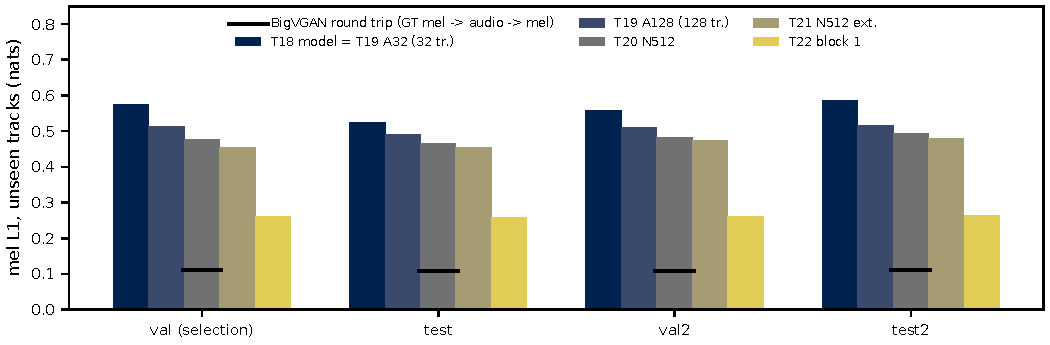
\includegraphics[width=\textwidth]{figures/heldout_progression.pdf}
\caption{\textbf{Unseen-track mel L1 across TASK-18--22} on identical crops (best checkpoints). Black ticks: BigVGAN round trip, a different metric shown for orientation only. Source: \src{artifacts/task20,21,22/analysis_v1/analysis.json}.}
\label{fig:heldout}
\end{figure}

\begin{figure}[t]
\centering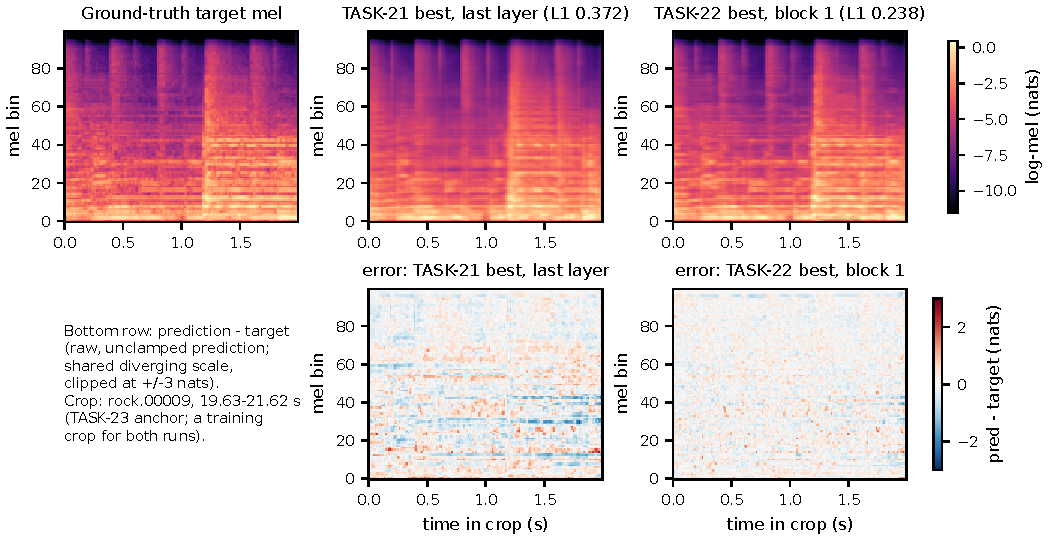
\includegraphics[width=\textwidth]{figures/anchor_depth.pdf}
\caption{\textbf{Same crop, two representations.} Ground truth, TASK-21 best (last layer) and TASK-22 best (block~1) on the anchor, with shared color scales. The anchor is a training crop for both runs, so this shows fit, not generalization.}
\label{fig:depth}
\end{figure}

\begin{figure}[t]
\centering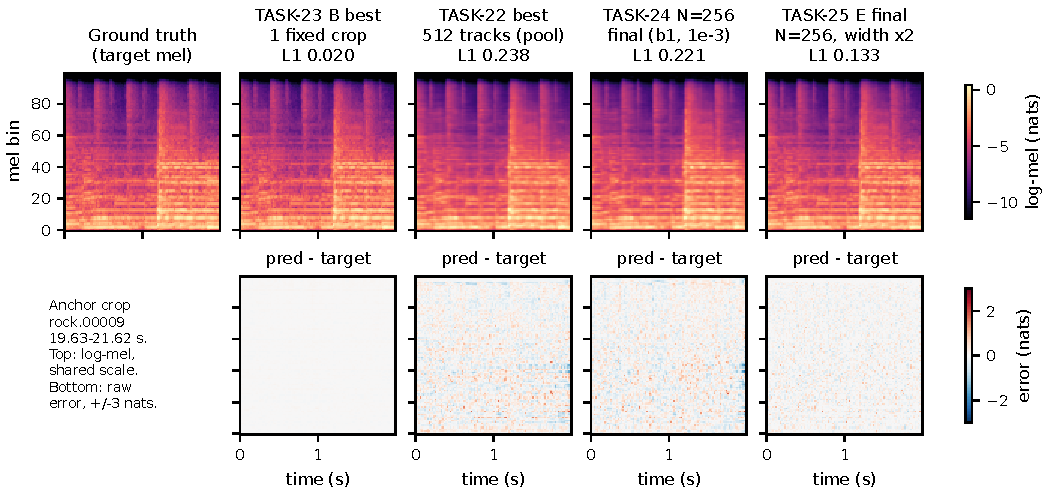
\includegraphics[width=\textwidth]{figures/anchor_regimes.pdf}
\caption{\textbf{Same crop under different fitting regimes,} with shared color scales. The one-crop fit (TASK-23) is visually indistinguishable from the target. Every multi-example model leaves broad, low-amplitude error and is smoother over time than the target.}
\label{fig:regimes}
\end{figure}

\paragraph{Temporal smoothness (descriptive statistic computed for this report).}
We define $V(m)=\mathrm{mean}|m_{:,t+1}-m_{:,t}|$, the mean frame-to-frame change of a mel.
\begin{itemize}
\item \obs\ On the anchor the target has $V=0.254$. TASK-23 B matches it (0.255). Every multi-example model is smoother: TASK-21 0.137, TASK-22 0.149, TASK-24 $N{=}256$ 0.150, TASK-25 C 0.171, E 0.167.
\item \obs\ On the 16 TASK-25 monitoring crops, the mean ratio $V(\hat y)/V(y)$ is lowest for the arms with the lowest monitoring error: D 0.57, F 0.58, A 0.63. It is highest for the arms with higher error: E 0.69, B 0.75, C 0.83.
\item \hyp\ Under L1, a translator uncertain about fine temporal detail may score better by predicting a smoothed mel than by committing to detail that is misplaced. This would fit both observations, but nothing here tests it, and L1 is not shown to cause the smoothing.
\end{itemize}

\begin{figure}[t]
\centering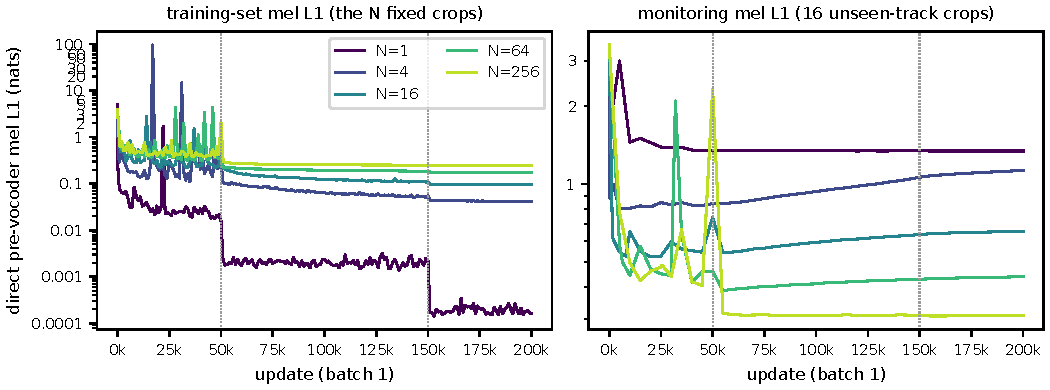
\includegraphics[width=\textwidth]{figures/task24_ladder.pdf}
\caption{\textbf{TASK-24 fitting ladder} (log scale; dotted: LR reductions at 50k and 150k). Left: error on each arm's own $N$ crops. Right: the 16 monitoring crops. Source: \src{runs/task24/task24_v1/N*/\{fit,monitor\}_eval.jsonl}.}
\label{fig:ladder}
\end{figure}

\begin{figure}[t]
\centering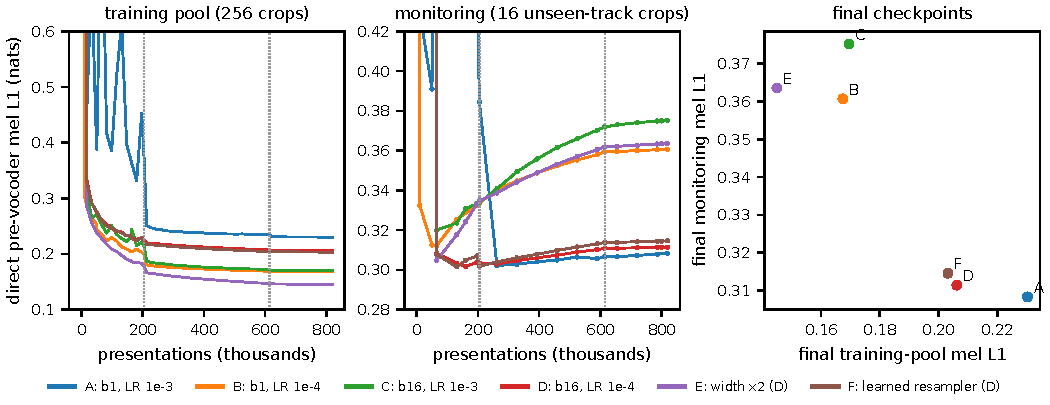
\includegraphics[width=\textwidth]{figures/task25_fit_vs_monitor.pdf}
\caption{\textbf{TASK-25: training fit vs monitoring.} Left and middle: whole-pool and monitoring mel L1 against presentations (dotted: LR reductions). Right: final checkpoints; the order of the two errors is exactly reversed. Source: \src{runs/task25/task25_v1/*/\{fit,monitor\}_eval.jsonl}.}
\label{fig:t25}
\end{figure}

% =====================================================================================================
\clearpage
\section{Synthesis: what could still limit reconstruction}
\label{sec:synthesis}
\begingroup\footnotesize
\setlength{\tabcolsep}{3pt}
\begin{longtable}{@{}L{2.3cm}L{4.8cm}L{4.4cm}L{4.6cm}@{}}
\toprule
Possibility & Evidence for & Evidence against & Untested\\
\midrule\endhead
\textbf{Representation accessibility / information} &
Depth changes recoverability by $\approx$43\% under a fixed decoder (T22). Even block 1 leaves held-out error at 0.26, with smoothed predictions. &
Every model beats every control (T18--22). Small pools memorize to 0.02--0.03, and shuffled conditioning then fails (1.06--2.03; T15). No experiment measures information loss. &
Other layers (\texttt{hidden\_states[0]}, 2--11); input normalization of the features; decoders able to undo the representation; the MuQ frontend mel itself as a control input.\\
\textbf{Decoder architecture / capacity} &
Fit error rises with $N$ (T24). Width $\times$2 lowers fit error by 0.061 at D's settings (T25). &
At $N{=}256$, optimization alone moves fit from 0.230 to 0.167. Width did not improve monitoring and was barely audible. &
Width at C's or B's settings; depth or receptive field; seeds; whether capacity helps when there are more tracks.\\
\textbf{Optimization} &
LR $\times$ batch interaction worth 0.06 (T25). Batch-1/LR $10^{-3}$ spikes (T15, T22--25). Early val optima (T18--20). &
Schedule B had no effect (T19). 47\,h of training gave only 2--3\% (T21). The second LR drop gives $\le2\%$ (T24, T25). &
Clipping; other optimizers; seeds. Plateaus under the tested schedules are not convergence.\\
\textbf{Data diversity / generalization} &
More tracks help held-out error with diminishing returns (T19, T20). More crops improve monitoring (T24). &
At 512 tracks block 1, train $\approx$ held-out error (T22), so the remaining error is mostly a fitting problem. In T25, better fit gave worse transfer at fixed $N$. &
More than 512 tracks; artist-aware splits; regularization or augmentation; seed variability of held-out gains.\\
\textbf{Objective / perceptual mismatch} &
Mel gains of 9--10\% (T19), 4--7\% (T20) and about 40\% on training crops (T25) are not audible. The temporal-smoothness observation (Sec.~\ref{sec:figs}). The cosine/MSE-saturation precedent from the codec line. &
One-crop L1 fits produce audio that matches the oracle (T15, T23), so L1 can drive perceptual fidelity when fitting succeeds. &
Error by band, transient vs sustained; perceptual or adversarial objectives; blinded rating of T22; whether mel L1 orders arms the way listeners do.\\
\textbf{Preprocessing / alignment} &
Isolated-crop context; whole-track peak gain set by outliers (anchor $\times$0.477 from a glitch at 7.18\,s); 3 edge-replicated frames per crop; 15--20\,ms misalignment existed until T16. &
The T16 fix changed little. Shuffled-time controls show coarse timing is correct. In the best-fitting T25 arms, boundary frames fit better than the interior (e.g.\ B 0.146 vs 0.169). &
Offset sweep of the alignment; whole-track vs isolated-crop extraction; per-crop vs per-track gain.\\
\textbf{Vocoder limitations} &
Round trip about 0.11 on every set; a weak click in BigVGAN($y$) on the anchor (cause unresolved). &
Ground-truth-mel audio is rated 3.9--4.0/4 (T19, T20). Memorized predictions sound like it (T15, T23). &
BigVGAN's sensitivity to smoothed or off-manifold mels: does it amplify or mask the translator's errors?\\
\bottomrule
\end{longtable}
\endgroup

\section{Discriminating next experiments}
\label{sec:next}
These are diagnostics that would separate the possibilities above, not a training plan. The first three need no training.
\begin{enumerate}
\item \textbf{Rate the existing TASK-22 blinded package.} Is a 43\% held-out mel gain audible, where 4--10\% gains were not?
\item \textbf{Decompose existing errors} by mel band, transient vs sustained frames, and boundary vs interior, together with $V(\hat y)/V(y)$. Use the saved TASK-22/24/25 predictions. Does the error sit mainly in temporal detail?
\item \textbf{Vocode controlled degradations of the true mel}: temporal smoothing matched to the observed $V$ ratios, and additive errors matched in L1. Listen blind. Does matching smoothness reproduce the perceived gap, and how much mel L1 is audible?
\item \textbf{Alignment offset sweep at evaluation time}: shift $p_j$ by $\pm$5--40\,ms for a saved checkpoint, with no retraining. Is the error minimal at zero offset?
\item \textbf{Seed replicates} of the TASK-25 contrasts that matter (C vs E; B vs C). Are the 0.02--0.06 effects larger than seed variability?
\item \textbf{Representation controls under one decoder}: the same translator fed \texttt{hidden\_states[0]} and MuQ's own input mel. How much of the gap between the last layer and block~1 is the frontend rather than the conformer?
\end{enumerate}

% =====================================================================================================
\appendix
\section{Detailed tables}
\label{app:tables}

\begin{table}[h]
\centering\footnotesize
\caption{TASK-22 window-best comparison (block 1 vs last layer). $\Delta$ = L12 $-$ L1 with 95\% track-clustered CI. Source: \src{artifacts/task22/analysis_v1/analysis.json}, \texttt{TASK-22\_ANALYSIS.md}.}
\begin{tabular}{@{}lccccc@{}}
\toprule
Set & round trip & L12 (step 60k) & L1 (step 193k) & $\Delta$ [95\% CI] & tracks L1 better\\
\midrule
val (selection) & 0.112 & 0.455 & 0.260 & 0.196 [0.166, 0.223] & 8/8\\
test & 0.109 & 0.454 & 0.257 & 0.198 [0.159, 0.252] & 8/8\\
val2 & 0.109 & 0.473 & 0.260 & 0.213 [0.192, 0.238] & 24/24\\
test2 & 0.111 & 0.480 & 0.263 & 0.217 [0.191, 0.249] & 24/24\\
unseen crops of training tracks (96) & 0.110 & 0.427 & 0.258 & 0.169 [0.160, 0.178] & 96/96\\
memorized (96) & 0.111 & 0.386 & 0.255 & 0.131 [0.126, 0.135] & 96/96\\
\bottomrule
\end{tabular}
\end{table}

\begin{table}[h]
\centering\footnotesize
\caption{TASK-25 final checkpoints (819{,}200 presentations each). Paired differences are over the 256 crops (bootstrap 95\% CI over crops); monitoring over 16 crops. Source: \src{artifacts/task25/task25_v1/ANALYSIS.md}, \texttt{report.json}.}
\begin{tabular}{@{}llcccccc@{}}
\toprule
Arm & Definition & Updates & Fit L1 & Anchor & Monitoring & Runtime & MACs/crop\\
\midrule
A & b1, LR $10^{-3}$ & 819{,}200 & 0.2303 & 0.208 & 0.308 & 39.0 min & 202\,M\\
B & b1, LR $10^{-4}$ & 819{,}200 & 0.1675 & 0.163 & 0.361 & 38.7 min & 202\,M\\
C & b16, LR $10^{-3}$ & 51{,}200 & 0.1696 & 0.170 & 0.375 & 3.5 min & 202\,M\\
D & b16, LR $10^{-4}$ (candidate) & 51{,}200 & 0.2062 & 0.187 & 0.311 & 3.4 min & 202\,M\\
E & width $\times$2, D settings & 51{,}200 & 0.1451 & 0.133 & 0.364 & 6.8 min & 771\,M\\
F & learned resampler, D settings & 51{,}200 & 0.2032 & 0.185 & 0.315 & 4.2 min & 208\,M\\
\midrule
\multicolumn{8}{@{}l}{Paired fit $\Delta$ (b$-$a): B$-$A $-0.063$ [$-0.065,-0.061$]; D$-$C $+0.037$ [0.035, 0.038]; C$-$A $-0.061$; D$-$B $+0.039$;}\\
\multicolumn{8}{@{}l}{E$-$D $-0.061$ [$-0.063,-0.060$]; F$-$D $-0.0030$ [$-0.0032,-0.0029$].}\\
\multicolumn{8}{@{}l}{Monitoring $\Delta$: B$-$A $+0.052$; D$-$C $-0.064$; E$-$D $+0.052$; F$-$D $+0.003$ [$-0.001$, 0.007].}\\
\bottomrule
\end{tabular}
\end{table}

\begin{table}[h]
\centering\footnotesize
\caption{TASK-20/21 training-track sets (core 32 tracks; best checkpoints unless stated). Source: \src{artifacts/task21/analysis_v1/analysis.json}.}
\begin{tabular}{@{}lccccc@{}}
\toprule
Set & A32 & A128 & T20 best & T21 best & T21 final\\
\midrule
memorized (64 crops) & 0.354 & 0.396 & 0.441 & 0.391 & 0.368\\
unseen crops of training tracks (64) & 0.451 & 0.448 & 0.464 & 0.439 & 0.446\\
\bottomrule
\end{tabular}
\end{table}

\paragraph{Runs and identifiers.}
\begin{itemize}
\item \textbf{TASK-15/16.} Local MPS; W\&B \texttt{seni7345}, \texttt{xl3nmbjt}, \texttt{fjh80gyn}. The commit is not recorded in the downloaded reports.
\item \textbf{TASK-18.} ACES 2240151, W\&B \texttt{274iituu}. The full-run commit is not in the downloaded report; the smoke run used \texttt{c6658b2} (dirty tree).
\item \textbf{TASK-19.} ACES 2244922--5, commit \texttt{2b4ef13}.
\item \textbf{TASK-20.} ACES 2246233, \texttt{dacda13}, W\&B \texttt{524aw8gs}.
\item \textbf{TASK-21.} ACES 2248110, \texttt{8a59c27}, W\&B \texttt{fxh15zi1}; 378.5 billing-hours.
\item \textbf{TASK-22.} ACES 2261697 (L1) and 2261638 (re-evaluation), commit \texttt{5e94361}.
\item \textbf{TASK-23.} ACES 2296013, \texttt{1cabc267}.
\item \textbf{TASK-24.} ACES 2296889, \texttt{766defc6}.
\item \textbf{TASK-25.} ACES 2299021, \texttt{4a2430e2}; W\&B \texttt{qht5cfn7}, \texttt{vug9tgcz}, \texttt{kdg6fvzy}, \texttt{yp2sin8w}, \texttt{mwegkdue}, \texttt{nxp8g38r}.
\end{itemize}

\section{Discrepancies between notes and code, resolved}
\label{app:discrepancies}
\begin{itemize}
\item \textbf{Pipeline description.} \src{CLAUDE.md} describes the EnCodec pipeline as current. TASK-15--25 use the BigVGAN-mel pipeline of Fig.~\ref{fig:pipeline}, as their configs and scripts show.
\item \textbf{Frame rate.} The ``25.07\,Hz'' in notes and reports is $50/1.9947$\,s, a finite-crop count. The implemented geometry uses the nominal 25\,Hz (960-sample hop).
\item \textbf{\texttt{encoder.py} docstring.} \texttt{encode\_all\_hidden\_states} says index $i\ge1$ is the output after block $i$ and that \texttt{hidden\_states[-1]} equals \texttt{last\_hidden\_state}. The second statement is right; the first is not exact for index 12, which includes the encoder LayerNorm (\src{task22.py}, hook-verified).
\item \textbf{\texttt{temporal\_conv.py} docstring.} It describes 1024 channels at the DAC frame rate (its origin in the codec experiments). In this pipeline the module runs with 256 channels at the 93.75\,Hz mel rate.
\item \textbf{MuQ depth.} The checkpoint's \texttt{w2v2\_config} lists 24 hidden layers, but \texttt{encoder\_depth: 12} overrides it; 12 layers are instantiated and 13 hidden states returned.
\item \textbf{Block-1/last-layer cosine.} The notes give 0.11 (TASK-22, over its crops); the anchor alone gives 0.097. These are different samples, not a conflict.
\item \textbf{TASK-18 reference numbers.} TASK-18's own report gives val 0.576 and test 0.525 (separate sets). TASK-19 tables pool primary val+test (0.550). Both are correct for their definitions.
\end{itemize}

\section{Reproducing this report}
Run from the repository root.
\begin{itemize}
\item \texttt{uv run python reports/task26\_pipeline\_report/scripts/inspect\_geometry.py --device cpu} writes \src{geometry.json}. It needs local MuQ weights and \src{third_party/} BigVGAN.
\item \texttt{uv run python reports/task26\_pipeline\_report/scripts/make\_figures.py} writes \src{figures/*.pdf} and \src{figure_data.json}. It needs the local TASK-21/22 checkpoints, TASK-23--25 predictions and logs.
\item Then \texttt{latexmk -pdf main.tex} inside \src{reports/task26_pipeline_report/}.
\end{itemize}
Neither script trains or writes outside the report directory.

\section{Unresolved facts}
\begin{itemize}
\item Git commits of TASK-15, TASK-16 and the TASK-18 full run are not in the local artifacts.
\item The source of the click shared by BigVGAN($y$) and every TASK-23 reconstruction of the anchor (vocoder, crop edge or other) is unresolved.
\item Listening is pending for TASK-16, TASK-22 (blinded package unrated) and TASK-24. TASK-21 has none. TASK-23 and TASK-25 listening was informal and unblinded.
\item Seed variability is unmeasured for every reported contrast.
\item The temporal localization of MuQ tokens after self-attention, and the effect of isolated-crop extraction on edge tokens, are unmeasured.
\item Whether the TASK-21 checkpoint behaves identically on the ACES-built features. The regenerated anchor error matched the recorded value to $7\times10^{-6}$, but only one crop was checked.
\end{itemize}

\bibliographystyle{plainnat}
\bibliography{refs}
\end{document}
